\chapter{Analyse und Auswertung}


\section{Testsystem}

Die Performanztests wurden auf folgendem System durchgeführt:


\section{Analyse mit Valgrind}

In diesem Abschnit wird auf die Analyse des Projektes mit Valgrind eingegangen. Zunächst werden Valgrind und die daraus benutzten Tools vorgestellt und dann werden einige Ergebnisse präsentiert.
\subsection{Valgrind}

Valgrind ist einerseits ein Framework zum Erzeugen von dynamsichen Analyse Werkzeugen und andereseits eine Sammlung ebensolcher Werkzeuge. 
Valgrind ist offene Software und wird unter der GNU GPL-2 Lizenz veröffentlicht\cite{valgrind}.

Valgrind is an instrumentation framework for building dynamic analysis tools. There are Valgrind tools that can automatically detect many memory management and threading bugs, and profile your programs in detail. You can also use Valgrind to build new tools.

The Valgrind distribution currently includes seven production-quality tools: a memory error detector, two thread error detectors, a cache and branch-prediction profiler, a call-graph generating cache and branch-prediction profiler, and two different heap profilers. It also includes an experimental SimPoint basic block vector generator. It runs on the following platforms: X86/Linux, AMD64/Linux, ARM/Linux, ARM64/Linux, PPC32/Linux, PPC64/Linux, PPC64LE/Linux, S390X/Linux, MIPS32/Linux, MIPS64/Linux, X86/Solaris, AMD64/Solaris, ARM/Android (2.3.x and later), ARM64/Android, X86/Android (4.0 and later), MIPS32/Android, X86/FreeBSD, AMD64/FreeBSD, X86/Darwin and AMD64/Darwin (Mac OS X 10.12).

Valgrind is Open Source / Free Software, and is freely available under the GNU General Public License, version 2.


\subsubsection{cachegrind und callgrind}
Cachegrind is a cache profiler. It performs detailed simulation of the I1, D1 and L2 caches in your CPU and so can accurately pinpoint the sources of cache misses in your code. It identifies the number of cache misses, memory references and instructions executed for each line of source code, with per-function, per-module and whole-program summaries. It is useful with programs written in any language. Cachegrind runs programs about 20--100x slower than normal.

Callgrind, by Josef Weidendorfer, is an extension to Cachegrind. It provides all the information that Cachegrind does, plus extra information about callgraphs. It was folded into the main Valgrind distribution in version 3.2.0. Available separately is an amazing visualisation tool, KCachegrind, which gives a much better overview of the data that Callgrind collects; it can also be used to visualise Cachegrind's output.
%\subsubsection{Memcheck}

%Gehört eigentlihc nciht wirklcih hier her
%Screenshot plus was macht das Tool. Wir haben das genutzt um sicherzustellen, dass es keine Memoryleaks gibt.

\subsubsection{Auswerten von callgrind-Ergebnissen}

Mithilfe der Anwendung QCachegrind können die Ergebnisse von Valgrinds cachegrind grafisch ausgewertet werden. QCachegrind ist ein Windowsbuild der Opensource Anwendung KCacheGrind.
KCachegrind ist vom Author des callgrind-Tools\cite{kcachegrind}.

TODO: Bildeinfügen und kurze erklärung


\section{Ergebnisse der Optimierungsmaßnahmen}

In diesem Abschnitt wird auf einige Ergebnisse der manuellen Performance-Messungen eingegangen.

\subsection{Hotpath}

Der häufigste Fall der Anwendung ist das Berechnen des Integrals in Situationen in denen keine Singularität auftritt. 
Dementsprechend werden diese in den implementierten Funktionen als der regelfall betrachtet.
Durch das vorziehen der Codestellen die diese Szenarien abhandeln werden beispielsweise die benötigten Sprunganweisungen geringer gehalten.
Eventuell Beispiel?



\subsection{Meistaufgerufene Funktion}
Die Funktion mit der größten Laufzeit ist das steepest-descent-Verfahren.
Diese Funktion ist über mehrere Iterationen optimiert worden, bis sie die im Kapitel \ref{Implementierung} dargestellte Form erreichte.
In früheren Versionen war dieses Verfahren in einer eigenen C++-Klasse implementiert, allerdings haben die Auswertungen gezeigt, dass ein
direkterer Aufruf der Gauss-Laguerre-Quadratur einen Laufzeitgewinn von fast 50 Prozent erzielen lies.

\subsection{Vermeiden von Funktionsaufrufen}

Bei der Implementierung des zweidimensionalen Falls\ref{2dint} hat sich gezeigt, dass das Nutzen der eindimenisionalen Implementierung zu erhöhten Laufzeiten geführt hat.

Samples: 50
Laguerre Punkte: 600
Auflösung: 0.1

Veränderung: läuft über resoltuion nicht K!s

Diese Messungen werden in der Abbildung \ref{abb_perf_indirect} dargestellt.

\begin{center}
  
\end{center}

Grafik folgt noch

\section{Auswertung der Laufzeitmessugen}

Die folgenen Laufzeitvergleiche wurden aus einer Matlab Umgebung heraus ausgeführt, d.h. es werden die ursprüngliche Implementierung sowie das Matlab-Modul der C++ Implementierung verglichen.


\subsection{Iteration über Wellenzahl}


In diesem Test wird die Laufzeit hinsichtlich veränderter Wellenzahl $k \in \{ 100, 500, 1000, 3000, 5000 \}$ gemessen.
Für jedes $k$ werden 50 zufällige Richtungsvektoren $r$ berechnet mit 600 Gauss-Laguerre-Knoten berechnet.

\begin{equation}
  A = \begin{pmatrix}
      0 & 0 \\
      1 & 0 \\
      0 & 1 \\
  \end{pmatrix}, b = \begin{pmatrix}
      0 \\ 0\\ 0
  \end{pmatrix},
\end{equation}

\begin{center}
    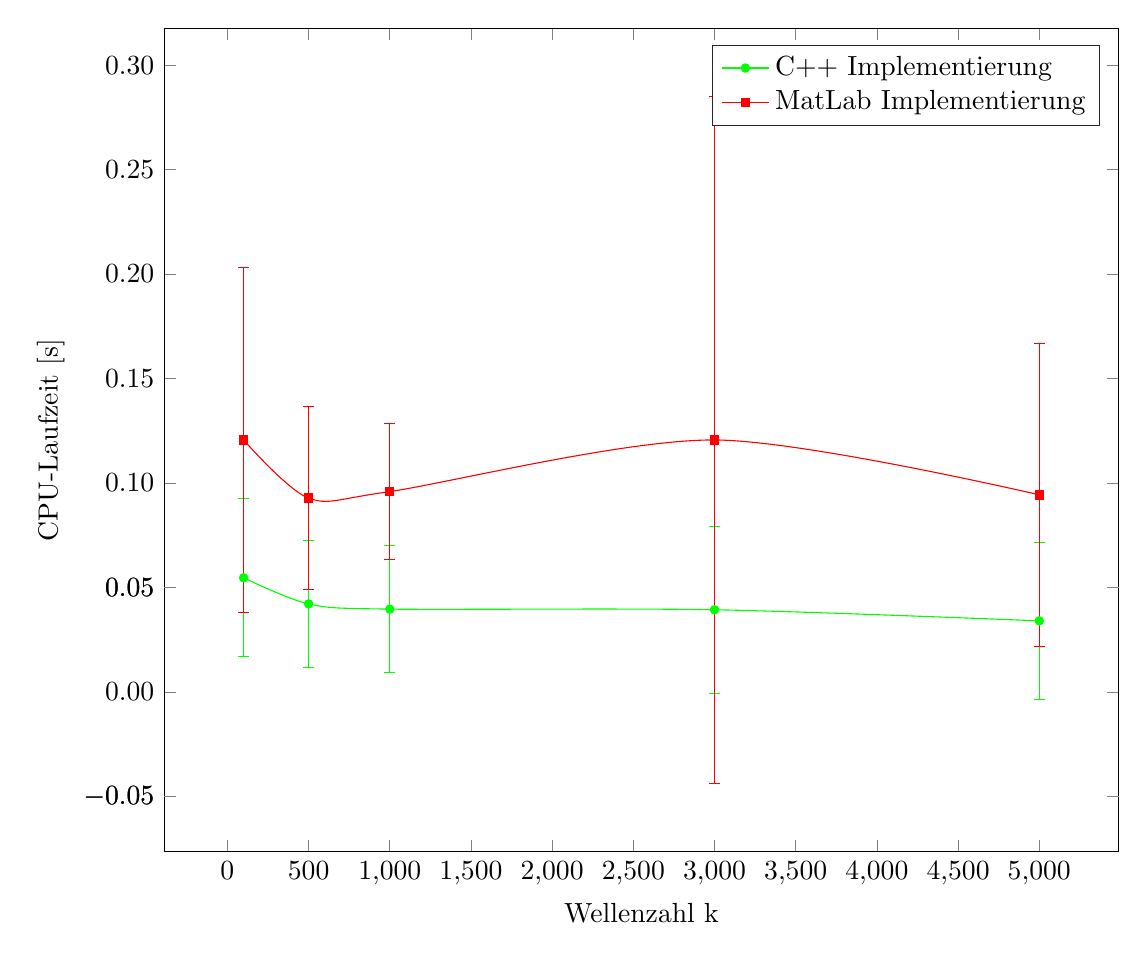
\begin{tikzpicture}
        \begin{axis}[
          width=\textwidth,
                  %width=3.358in,
        %height=2.309in,
        %at={(0.563in,0.312in)},
        scale only axis,
        yticklabel style={
          /pgf/number format/fixed,
          /pgf/number format/precision=2,
          /pgf/number format/fixed zerofill
        },
        extra y ticks={-0.05, 0.05},
        scaled y ticks=false,
        xlabel=Wellenzahl k,
        ylabel=\text{CPU-Laufzeit [s]},
        %xmin=0,
       % xmax=6000,
        %ymin=0,
        %ymax=0.5,
        axis background/.style={fill=white},
        legend style={legend cell align=left, align=left, draw=white!15!black}
        ]
        \addplot+[
      green, mark options={green, scale=0.75},
      smooth, 
      error bars/.cd, 
        y fixed,
        y dir=both, 
        y explicit ] table [color=green, mark=o, mark options={solid, green} x=k, y=t,y error=std, col sep=comma] { 
            k, t, std 
            100, 0.0546875000000000, 0.0377819439281490
            500, 0.0421875000000000, 0.0304832595619367
            1000, 0.0396875000000000, 0.0304767208961468
            3000, 0.0393750000000000, 0.0399597214296433
            5000, 0.0340625000000000, 0.0374428241844571         
          };
          \addplot+[
            red, mark options={red, scale=0.75},
            smooth, 
            error bars/.cd, 
              y fixed,
              y dir=both, 
              y explicit ] table [color=red, mark=o, mark options={solid, red} x=k, y=t,y error=std, col sep=comma] { 
                  k, t, std 
                  100, 0.120625000000000, 0.0825011595465820
                  500, 0.0928125000000000, 0.0439012055439740
                  1000, 0.0959375000000000, 0.0326549607327770
                  3000, 0.120625000000000, 0.164181352722021
                  5000, 0.0943750000000000, 0.0724645849462240          
                };
        %\addplot [color=red, draw=none, mark=o, mark options={solid, mycolor1}]
        %  table[row sep=crcr] file {..\data\performance_matlab.csv};
        \addlegendentry{C++ Implementierung}
        \addlegendentry{MatLab Implementierung}

        \end{axis}
    \end{tikzpicture}%
    \captionof{figure}{Laufzeitvergleich über verschiedene Wellenzahlen $k$}
\end{center}


\subsection{Laufzeitvergleich bei steigender Auflösung}


In diesem Test wird die Laufzeit hinsichtlich veränderter Auflösung $res \in \{ 0.1, 0.01, 0.001, 0.0001 \}$ gemessen.
Für jedes $k$ werden 50 zufällige Richtungsvektoren $r$ berechnet mit 600 Gauss-Laguerre-Knoten berechnet.

\begin{equation}
  A = \begin{pmatrix}
      0 & 0 \\
      1 & 0 \\
      0 & 1 \\
  \end{pmatrix}, b = \begin{pmatrix}
      0 \\ 0\\ 0
  \end{pmatrix},
\end{equation}
    
\begin{center}
    \begin{tikzpicture}
        \begin{axis}[
        %width=3.358in,
        %height=2.309in,
        %at={(0.563in,0.312in)},
        scale only axis,
        xmode=log,
        ymode=log,
        ymax=1000,
        width=\textwidth,
        %log ticks with fixed point,
        x dir=reverse,
        ylabel=\text{CPU-Laufzeit [s] (log)},
        xlabel=Layer-Auflösung (log),
        % for log axes, x filter operates on LOGS.
        % and log(x * 1000) = log(x) + log(1000):
        %x filter/.code=\pgfmathparse{#1 + 6.90775527898214},
        axis background/.style={fill=white},
        legend style={legend cell align=left, align=left, draw=white!15!black}
        ]
        \addplot+[
      green, mark options={green, scale=0.75},
      smooth, 
      error bars/.cd, 
        y fixed,
        y dir=both, 
        y explicit ] table [color=green, mark=o, mark options={solid, green} x=res, y=t,y error=std, col sep=comma] { 
            res, t, std
            0.1000,    0.0563,    0.0461
            0.0100,    0.3469,    0.0645
            0.0010,   3.8547,    1.6996
            0.0001,  38.9781,   15.6876
          };
          \addplot+[
            red, mark options={red, scale=0.75},
            smooth, 
            error bars/.cd, 
              y fixed,
              y dir=both, 
              y explicit ] table [color=red, mark=o, mark options={solid, red} x=res, y=t,y error=std, col sep=comma] { 
                  res, t, std
                  0.1000,    0.1375,    0.0799
                  0.0100,    0.8688,    0.0834
                  0.0010,    9.5406,    4.2787
                  0.0001,   86.2375,   27.7633
                };
        %\addplot [color=red, draw=none, mark=o, mark options={solid, mycolor1}]
        %  table[row sep=crcr] file {..\data\performance_matlab.csv};
        \addlegendentry{C++ Implementierung}
        \addlegendentry{MatLab Implementierung}
        \end{axis}
    \end{tikzpicture}%
    \captionof{figure}{Laufzeitvergleich über verschiedene Auflösungen, logarithmische Skalen}
\end{center}


\section{Vergleiche der relativen Genauigkeit}

